%======================================================================
\chapter{Architecture}
%======================================================================
\label{ch:arch}

\begin{figure}[b!]
\centering
  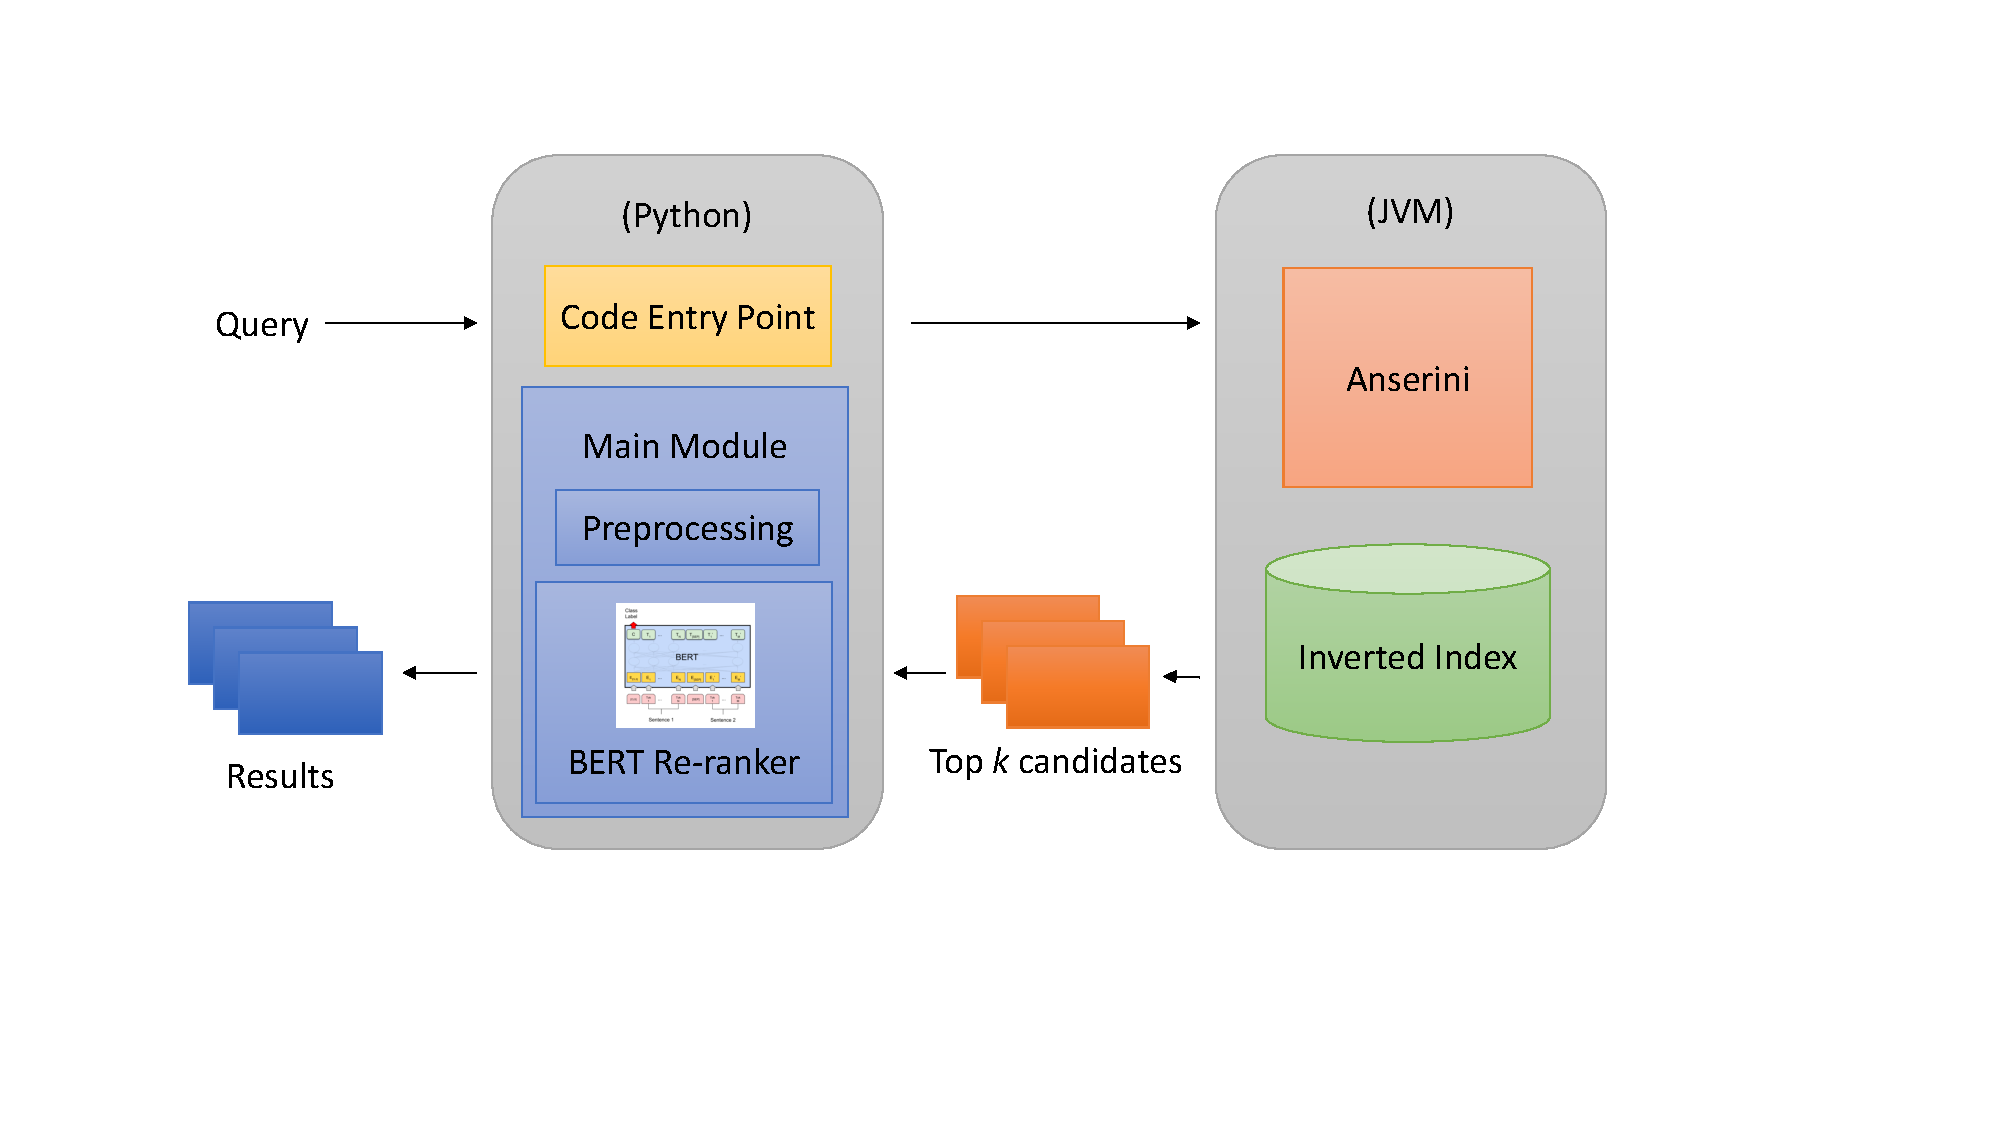
\includegraphics[width=5in]{figures/architecture.pdf}
\caption{Architecture of our system featuring tight integration between Python and the JVM.}
\label{fig:arch}
\end{figure}

In this chapter, we detail the architecture that allows us to employ the model introduced in Chapter~\ref{ch:model}, review each component of the architecture and discuss the design choices behind their integration.
We also touch upon the issue of reproducibility in information retrieval and our efforts to make our work more reproducible as well as their current limitations.

We apply BERT to document retrieval via integration with the open-source information retrieval toolkit Anserini.\footnote{\url{http://anserini.io}}
The architecture of our system, Birch, follows a two-stage pipeline as shown in Figure \ref{fig:arch}:\
Anserini is used to retrieve documents from indexed collections with BM25, forming an initial candidate list.
Our BERT-based model is deployed as a re-ranker over the candidate documents to produce a final ranking of documents based on sentence-level relevance.
%\myworries{Does this make sense: These parts can be divided into two main categories based on their medium of execution:\ Python and JVM.}

\section{Anserini}

Technology transfer between the academic and industrial information retrieval communities is at times impeded due to a lack of universal set of tools and infrastructure.
Most industry practitioners have adopted Lucene,\footnote{\url{https://lucene.apache.org}} Solr,\footnote{\url{https://lucene.apache.org/solr}} or Elasticsearch\footnote{\url{https://www.elastic.co}} as the de facto platform in the development of search applications with the primary objective of scalability.
However, academic systems such as Indri\footnote{\url{https://www.lemurproject.org}} and Terrier,\footnote{\url{http://terrier.org}} which prioritize better rankings above all else with little consideration for operational characteristics, are far more prevalent among researchers.

Anserini~\cite{Yang_etal_SIGIR2017} was developed in response to this disconnect to provide a research-focused information retrieval toolkit on top of the open-source Lucene search library.
Anserini facilitates efficient full text indexing and search capabilities over large-scale text collections by providing wrappers and intuitive APIs on top of core Lucene libraries.
More importantly, Anserini makes it possible for researchers and industry practitioners alike to systematically evaluate their models over standard test collections in a reproducible and comparable manner.

Related to our work, Anserini can be seamlessly integrated into multi-stage ranking architectures with large improvements in retrieval effectiveness and low latency as demonstrated by Nogueira et al.~\cite{nogueira2019passage} and Yang et al.~\cite{yang2019end}.
Similar to their work, we initially use Anserini to index our test collections in a multi-threaded manner with Lucene 8.0 (post commit id \texttt{75e36f9}).
% \myworries{which has greatly improved query evaluation latency over the previous Lucene 7.6}).
For each test collection, we retrieve an initial ranked list of documents 1000 for each query with BM25 with RM3 query expansion using default Anserini parameters.

%\myworries{Is this part necessary? How can it be modified?}
%Anserini has already been successfully adopted in multiple projects:\
%For example, \cite{nogueira2019passage} used Anserini for generating candidate documents before applying BERT to ranking passages in the TREC Complex Answer Retrieval (CAR) task~\cite{dietz2017trec}, which led to a large increase in effectiveness.
%\cite{Yang_etal_arXiv2019} also combined Anserini and BERT to demonstrate large improvements in open-domain question answering directly on Wikipedia.

\section{Main Module}

%\myworries{Need a better name that doesn't include Python...}
The main Python module lies at the core of our system, encompassing the preprocessing, training / inference and evaluation components.
All the functionalities of our proposed model discussed in Chapter \ref{ch:model} are implemented in this module in Python using the deep learning framework PyTorch.\footnote{\url{https://pytorch.org}}

The preprocessing component of this module consumes the documents retrieved with Anserini, and converts them into a format that can be used by the main component that enables training and inference with BERT.
On the one hand, the main component can be used to train BERT as a relevance classifier.
This functionality may be used independently of the overall pipeline to fine-tune BERT on new collections.
On the other hand, we can run inference over the output of the preprocessing module with previously trained models, producing a list of sentence relevance scores.
This component also serves as a re-ranker where sentence and BM25 document scores are interpolated in order to compute an overall relevance score for each candidate document.
The evaluation component uses the $\texttt{trec\_eval}$ tool to assess the retrieval effectiveness of our system.

\section{Integration}

Our two-stage pipeline marries NLP and IR capabilities to implement a document retrieval system that successfully leverages semantic cues in documents.
For an effective integration, we need to address the the technical challenge of connecting the two components that have fundamentally different infrastructural requirements.
In this section we discuss the design choices in bridging the worlds of NLP and IR from a software engineering viewpoint.

Anserini, which is responsible for indexing and retrieval in our system, runs on the Java Virtual Machine (JVM) as it is mostly implemented in Java or provides Python wrappers on Java.
However, our deep learning framework of choice PyTorch, similar to alternatives such as TensorFlow,\footnote{\url{https://www.tensorflow.org}} are implemented in Python with a C\texttt{++} backend.
% to support blah

There exist two immediate solutions to connecting Python and the JVM.
``Loosely-coupled'' integration approaches involve using an intermediary medium between Python and the JVM.
For example, we may pass text files between the two in order to facilitate communication without direct interaction.
However, this is not an efficient solution as it requires writing/reading potentially large files to/from disk, not to mention the memory requirements.
Furthermore, this approach requires diligent monitoring to ensure that changing file formats and APIs do not break code.
Integration via REST APIs is plagued with similar issues as passing intermediate text files.
Specifically, it may require frequent HTTP calls, thus introducing significant overhead.
Additionally, imperfect solutions for enforcing API contracts risk stability of the system.
Ultimately, neither approach is suitable for rapid experimentation in a research environment.

Therefore, we explore ways to achieve ``tightly-coupled'' integration.
One solution is to adopt the Java Virtual Machine (JVM) as the primary code entry point, and connect to PyTorch's C\texttt{++} backend via the Java Native Interface (JNI).
However, this would result in two separate code paths (JVM to C\texttt{++} for execution and Python to C\texttt{++} for model development), leading to maintainability issues similar to those mentioned with regard to REST APis.

For this reason, we finally chose Python as our primary development environment, integrating Anserini using the Pyjnius Python library\footnote{\url{https://pyjnius.readthedocs.io}} for accessing Java classes.
Pyjnius was originally developed to facilitate Android development in Python, and allows Python code to directly manipulate Java classes and objects.
Thus, our system supports Python as the main development language (and code entry point, as shown in Figure~\ref{fig:arch}), connecting to the JVM to access retrieval capabilities of Anserini.

\section{Replicability and Reproducibility}

Over the last decade, it has become increasingly challenging to verify reported results and compare various performance metrics due to growing number of information retrieval systems both in academia and the industry.
Unlike some fields of computer science where it is practical to manually corroborate findings or visually inspect results, the amount and type of data involved in document retrieval deems this approach infeasible.
This challenge has prompted one of the largest IR conferences in the world, SIGIR, to issue a task force to determine guidelines to establish repeatability, replicability, and reproducibility principles in IR projects.\footnote{\url{http://sigir.org/wp-content/uploads/2018/07/p004.pdf}}

\newpage

The first dimension of this movement, repeatability, emphasises a researcher's ability to reliably repeat her own runs.
The path to this goal is through rigorous logging, good data management practices and consistent use of virtual environments.
We do not delve further into the details of repeatability as the practices we follow are universal to all research endeavors.

The second dimension, replicability, highlights the ability of an independent group to obtain the same results using the researcher's original artifacts.
We strive to make our work replicable by building a Docker image to accompany our system that allows anyone to deploy and test our system on any operating system easily.
By adhering to the requirements defined in the SIGIR Open-Source IR Replicability Challenge (OSIRRC), we ensure that our system can seamlessly work with their evaluation infrastructure in the future.
%\myworries{The image is available on Docker hub with the tag \texttt{tag}.}
The OSIRRC jig\footnote{\url{https://github.com/osirrc/jig}} needs to be set up first to run the commands on Docker hub.
The OSIRRC Docker container contract includes three ``hooks'' for interacting with the system:\
the \texttt{init} hook has to be called first, whose purpose is to run any preparatory steps for the retrieval run including downloading and compiling the source code, downloading pre-built artifacts such as JAR files and other external resources such as pretrained models.
In our case, we pull the source code, data and pretrained models from Google Cloud Storage buckets; build Anserini with Maven, and the $\texttt{trec\_eval}$ tool.
Next the \texttt{index} hook is called to, as the name indicates, build the necessary indexes.
Finally, the \texttt{search} hook performs multiple ad-hoc retrieval runs in a row.
Since the GPU hooks necessary for inference with BERT have not been implemented yet, \texttt{search} relies on pre-computed sentence scores instead of obtaining them from scratch.
Each of the hook scripts accepts a JSON file that defines the various arguments for the respective script such as path to the relevance judgments file.

Finally, the third dimension, reproducibility, refers to the the ability of an independent group of researchers to implement the author's proposed artifacts from scratch with the same results.
This final goal is indeed the hardest to achieve; as a matter of fact, it may even be impossible in certain cases due to non-determinism.
Unfortunately, we found this to be true with some aspects of our work with BERT as well.
For example, the fine-tuning and inference processes described in Chapter~\ref{ch:model} produces slightly different sentence scores (i.e., third decimal) unless they are performed on the same GPU.
To further aggravate this issue, these small differences add up over floating point operations, leading to as much as a 0.5 point difference in AP.
We try to relieve this issue by releasing our tuned hyperparameters which help reproduce the same results despite minor differences in sentence scores, and by reporting results for runs on the same GPU.
We intend to study this issue further and come up with a systematic solution in future work.

%\myworries{Score ties, hyperparameters?}

%Score ties are currently broken in hyperparameter tuning by picking the smaller of numbers.

%A number of frameworks that help machine learning researchers keep track of their experiments, such as Sacred\footnote{https://github.com/IDSIA/sacred} and Forge\footnote{https://github.com/akosiorek/forge}, have emerged over the last few years.
%By adding only a few lines of code, these frameworks save and display the details of each experiments on an online dashboard so that the researcher can go back and reproduce her experiments easily.

%Similar to the Google Colab notebook, the Docker image is restricted to experiments with $ \textrm{BERT}_{\textrm{\scriptsize Base}}(\textrm{MB})$ on Robust04 for the sake of simplicity.

%difficult to put progress on solid footing
%in terms of software engineering best practices, since developers
%cannot be certain if a new feature introduced a bug
%
% However,
%the interaction between multi-threaded indexing and score ties
%during retrieval may yield non-deterministic rankings, making repeatability not as trivial as one might imagine. In the context of
%the open-source Lucene search engine, score ties are broken by
%internal document ids, which are assigned at index time. Due to
%multi-threaded indexing, which makes experimentation with large
%modern document collections practical, internal document ids are
%not assigned consistently between different index instances of the
%same collection, and thus score ties are broken unpredictably. This
%short paper examines the effectiveness impact of such score ties,
%quantifying the variability that can be attributed to this phenomenon. The obvious solution to this non-determinism and to ensure
%repeatable document ranking is to break score ties using external
%collection document ids. This approach, however, comes with measurable efficiency costs due to the necessity of consulting external
%identifiers during query evaluation.

%\section{Other Integrations}
%\myworries{HiCAL? Colab? does that even make sense?}